\documentclass{beamer}

\mode<presentation> {
\usetheme{AnnArbor}
}

\usepackage{graphicx}
\graphicspath{{./figures/}}
\usepackage{caption}
\usepackage{subcaption}
\usepackage{hyperref}
\hypersetup{colorlinks=true}
\usepackage{amsmath}
\usepackage{amsthm}
\usepackage{biblatex}
\addbibresource{bibliography.bib}

\title[Univariate Extreme Value Theory]{Univariate Extreme Value Theory}

\author{Victor Verma}
\institute[]
{
Prof. Yang Chen's Reading Group \\
Department of Statistics \\
University of Michigan
}
\date[1/26/23]{1/26/23} 

\begin{document}

\begin{frame}
    \titlepage
\end{frame}

\begin{frame}{Today's Reading}
    \begin{itemize}
        \item Chapter 3 of \textit{Modelling Extremal Events} by Embrechts, Kl\"{u}ppelberg, and Mikosch (\cite{embrechts_et_al_1997})
    \end{itemize}
\end{frame}

\begin{frame}{Outline}
    \tableofcontents
\end{frame}

\begin{frame}{An Example Problem}
    \begin{figure}
        \centering
        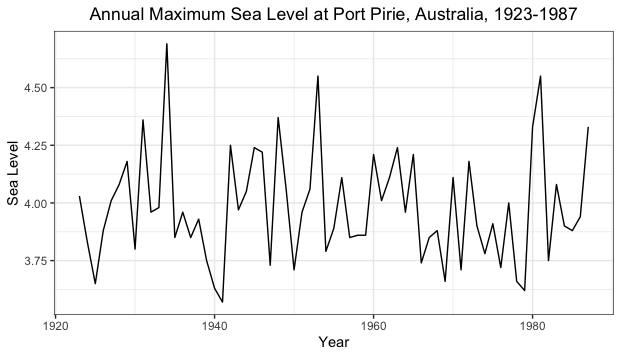
\includegraphics[scale=0.5]{max_sea_levels.png}
        \caption{Annual maximum sea levels at Port Pirie, Australia, 1923-1987.}
        \label{fig:max_sea_levels}
    \end{figure}    
\end{frame}

\begin{frame}{An Example Problem}
    Some questions:
    \begin{itemize}
        \item What sea level is observed once every 100 years? every 1,000 years?
    \end{itemize}

    A necessary assumption:
    \begin{itemize}
        \item Current climactic conditions will persist
    \end{itemize}

    \bigskip
    
    Some terminology:
    \begin{itemize}
        \item An event with probability $p$ has \textbf{return period} $1 / p$
        \item The \textbf{return level} with return period $1 / p$ is the upper $p$th quantile of the distribution
    \end{itemize}
    The annual maximum sea level observed once every 100 years is the return level with return period $1 / 100 = 0.01$.
\end{frame}

\begin{frame}{An Example Problem}
    Some notation:
    \begin{itemize}
        \item Let $X \sim F$ be the sea level on a day.
        \item Let $M_n = \max_{i = 1, \ldots, n} X_i$ be the maximum over a period of $n$ days.
    \end{itemize}
    The return level with return period 0.01 is $m_{0.01}$, the upper 0.01 quantile of $F^{365}$, the df of $M_{365}$.

    \bigskip

    How to estimate $m_{0.01}$?
\end{frame}

\begin{frame}{An Example Problem}
    One idea:
    \begin{itemize}
        \item Approximate $F$ by $\hat{F}$, then approximate $F^{365}$ by $\hat{F}^{365}$.
        \begin{itemize}
            \item The error in $\hat{F}$ will get compounded.
        \end{itemize}
    \end{itemize}

    Another idea:
    \begin{itemize}
        \item Directly approximate $F^{365}$ using the the asymptotic behavior of $M_n$.
        \item If $F^n \xrightarrow{d} G$ for some df G, then $F^n \approx G$ for large $n$, like 365.
    \end{itemize}
\end{frame}

\begin{frame}{The Block Maximum Approach}
    $M_n$ is a \textbf{block maximum}. The block maximum approach to extreme value analysis:
    \begin{itemize}
        \item Divide data $X_1, X_2, X_3, \ldots \overset{\text{iid}} F$ into blocks of size $n$
        \item Find a $G$ such that $F^n \xrightarrow{d} G$.
        \item Use $G$ to approximate $F^n$ for $n$ of interest
    \end{itemize}
\end{frame}

\begin{frame}{The Block Maximum Approach, First Attempt}
    The \textbf{right endpoint} of $F$ is
    \begin{align*}
    x_F &= \sup\{x \in \mathbb{R} : F(x) < 1\} \\
    &= \inf\{x \in \mathbb{R} : F(x) = 1\}
    \end{align*}
    If $x_F < \infty$, then $M_n \xrightarrow{d} x_F$. $F_{x_F}$ is a bad approximation to $F^n$ because it is \textbf{degenerate}.

    \bigskip

    What to do?
\end{frame}

\begin{frame}{The Block Maximum Approach, Second Attempt}
    In the CLT, $S_n = \sum_{i = 1}^n X_i$ is \textbf{normalized}:
    \[
    \frac{1}{\sigma\sqrt{n}}(S_n - n\mu) \xrightarrow{d} N(0, 1)
    \]
    Idea: Normalize $M_n$ - consider $c_n^{-1}(M_n - d_n)$ as $n \to \infty$ for some $c_n > 0$ and $d_n$. If $c_n^{-1}(M_n - d_n) \xrightarrow{d} G$ and $G$ is nondegenerate, then for large $n$,
    \begin{align*}
        F^n(x) &= P(M_n \le x) \\
        &= P(c_n^{-1}(M_n - d_n) \le c_n^{-1}(x - d_n)) \\
        &\approx G(c_n^{-1}(x - d_n)).
    \end{align*}
\end{frame}

\begin{frame}{Limit Probabilities for Maxima}
    We have
    \[
    P(c_n^{-1}(M_n - d_n) \le x) = P(M_n \le c_n x + d_n)
    \]
    We want $P(M_n \le c_n x + d_n) \to G(x)$ for some nondegenerate df $G$. We can consider $\lim_{n \to \infty} P(M_n \le u_n)$ for arbitrary sequences $\{u_n\}$.
    
    \bigskip
    
    Question: \textit{which conditions on $F$ ensure that $\lim_{n \to \infty} P(M_n \le u_n) \in (0, 1)$ for some $\{u_n\}$?}
\end{frame}

\begin{frame}{Limit Probabilities for Maxima}
    The \textbf{tail} $\bar{F}$ of a distribution function $F$ is $1 - F$.
    \begin{corollary}[3.1.2]
        Suppose that $x_F < \infty$ and $F(x_F-) < 1$. Then for every sequence $\{u_n\}$ such that $P(M_n \le u_n) \to \rho$, either $\rho = 0$ or $\rho = 1$.
    \end{corollary}
    \begin{theorem}[3.1.3]
        Let $F$ be a df with right endpoint $x_F \le \infty$ and let $\tau \in (0, \infty)$. There exists a sequence $\{u_n\}$ satisfying $n\bar{F}(u_n) \to \tau$ if and only if
        \[
        \lim_{x \uparrow x_F} \frac{\bar{F}(x)}{\bar{F}(x-)} = 1
        \]
        and $F(x-) = 1$.
    \end{theorem}
\end{frame}

\begin{frame}{Limit Probabilities for Maxima}
    Corollary 3.1.2 and Theorem 3.1.3 rule out
    \begin{itemize}
        \item The binomial distribution
        \item The Poisson distribution
        \item The geometric distribution
        \item The negative binomial distribution
    \end{itemize}
\end{frame}

\begin{frame}{Weak Convergence of Maxima Under Affine Transformations}
    Question: \textit{what are the possible nondegenerate limit laws for the maxima $M_n$ when properly normalized?}
\end{frame}

\begin{frame}{The Fisher-Tippett Theorem, Version 1}
    \begin{theorem}[Fisher-Tippett]
        Let $\{X_n\}$ be a sequence of iid rvs. If there exist norming constants $c_n > 0$, $d_n \in \mathbb{R}$ and some non-degenerate df $G$ such that $c_n^{-1}(M_n - d_n) \xrightarrow{d} G$, then $G$ belongs to one of the following families:
        \begin{align*}
            \text{(Fr\'{e}chet)} \quad \Phi_{\alpha}(x) &=
            \begin{cases}
                0, & x \le b \\
                \exp\left\{-\left(\frac{x - b}{a}\right)^{-\alpha}\right\}, & x > b
            \end{cases} \\
            \text{(Weibull)} \quad \Psi_{\alpha}(x) &=
            \begin{cases}
                \exp\{-\left[-\left(\frac{x - b}{a}\right)\right]^{\alpha}\}, & x < b \\
                1, & x \ge b
            \end{cases} \\
            \text{(Gumbel)} \quad \Lambda(x) &= \exp\left\{-e^{-\left(\frac{x - b}{a}\right)}\right\}, \qquad x \in \mathbb{R}
        \end{align*}
        for parameters $a > 0$, $b$, and $\alpha > 0$.
    \end{theorem}
\end{frame}

\begin{frame}{The GEV Distribution}
    The Fr\'{e}chet, Weibull, and Gumbel distributions are special cases of the \textbf{GEV distribution}:
    \[
    G(z) = \exp\left\{-\left[1 + \xi\left(\frac{z - \mu}{\sigma}\right)\right]^{-1 / \xi}\right\},
    \]
    defined on $\{z : 1 + \xi(z - \mu) / \sigma > 0\}$, where $\mu \in \mathbb{R}$, $\sigma > 0$, and $\xi \in \mathbb{R}$.

    \begin{itemize}
        \item $\xi > 0$: Fr\'{e}chet
        \item $\xi < 0$: Weibull
        \item $\xi = 0$: Gumbel
    \end{itemize}

    \medskip

    Using the GEV distribution is preferred in modeling.
\end{frame}

\begin{frame}{The Fisher-Tippett Theorem, Version 2}
    \begin{theorem}[Fisher-Tippett]
        Let $\{X_n\}$ be a sequence of iid rvs. If there exist norming constants $c_n > 0$, $d_n \in \mathbb{R}$ and some non-degenerate df $G$ such that $c_n^{-1}(M_n - d_n) \xrightarrow{d} G$, then $G$ belongs to the GEV family:
        \[
        G(z) = \exp\left\{-\left[1 + \xi\left(\frac{z - \mu}{\sigma}\right)\right]^{-1 / \xi}\right\}
        \]
        defined on $\{z : 1 + \xi(z - \mu) / \sigma > 0\}$, where $\mu \in \mathbb{R}$, $\sigma > 0$, and $\xi \in \mathbb{R}$.
    \end{theorem}
\end{frame}

\begin{frame}{The Block Maximum Approach}
    Idea: Normalize $M_n$ - consider $c_n^{-1}(M_n - d_n)$ as $n \to \infty$ for some $c_n > 0$ and $d_n$. If $c_n^{-1}(M_n - d_n) \xrightarrow{d} G$ and $G$ is nondegenerate, then for large $n$,
    \begin{align*}
        F^n(x) &= P(M_n \le x) \\
        &= P(c_n^{-1}(M_n - d_n) \le c_n^{-1}(x - d_n)) \\
        &\approx G(c_n^{-1}(x - d_n)).
    \end{align*}
    $G(x)$ is GEV; so is $G(c_n^{-1}(x - d_n))$.
\end{frame}

\begin{frame}{Max-Stability}
    \begin{definition}
        A non-degenerate rv $X$ (the corresponding distribution or df) is called \textbf{max-stable} if for every $n \ge 2$, iid $X, X_1, \ldots, X_n$, appropriate constants $c_n > 0$ and $d_n \in \mathbb{R}$ it satisfies
        \[
        \max\{X_1, \ldots, X_n\} \overset{d}{=} c_n X + d_n
        \]
    \end{definition}
    Important fact: \textit{A distribution is max-stable if and only if it is a limit distribution for maxima of iid rvs.}
    Prove this using the proof of Theorem 3.2.2 of \cite{embrechts_et_al_1997}.
\end{frame}

\begin{frame}{Type}
    \begin{definition}
        We say that X and Y (and the corresponding distributions and dfs) belong to the same type or are of the same type if there exist constants $a \in R$ and $b > 0$ such that $X \overset{d}{=} b Y + a$.
    \end{definition}
\end{frame}

\begin{frame}{Convergence to Types Theorem}
    \begin{theorem}[Convergence to Types Theorem]
        Let $A, B, A_1, A_2, \ldots$ be rvs and $b_n > 0$, $\beta_n > 0$ and $a_n, \alpha_n \in \mathbb{R}$ be constants. Suppose that
        \[
        b_n^{-1}(A_n - a_n) \xrightarrow{d} A.
        \]
        Then the relation
        \[
        \beta_n^{-1}(A_n - \alpha_n) \xrightarrow{d} B \tag{1}
        \]
        holds if and only if
        \[
        \lim_{n \to \infty} b_n / \beta_n = b \in [0, \infty), \lim_{n \to \infty} (a_n - \alpha_n) / \beta_n = a \in R. \tag{2}
        \]
        If (1) holds then $B \overset{d}{=} b A + a$ and $a, b$ are the unique constants for which this holds. When (1) holds, $A$ is non–degenerate if and only if $b > 0$, and then $A$ and $B$ belong to the same type.
    \end{theorem}
\end{frame}

\begin{frame}{The Fisher-Tippett Theorem: Proof Sketch}
    Use the sketch of the proof of Theorem 3.2 of \cite{coles_2001}.
\end{frame}

\begin{frame}{Inference for the Block Maximum Approach}
    Assume that block maxima $Y_1, \ldots, Y_k$ are iid GEV.

    \medskip
    
    If $\xi \ne 0$, the log-likelihood is
    \begin{align*}
        \ell(\mu, \sigma, \xi) &= -k\log\sigma \\
        &\quad - (1 + 1 / \xi)\sum_{i = 1}^k \log\left[1 + \xi\left(\frac{y_i - \mu}{\sigma}\right)\right] \\
        &\quad - \sum_{i = 1}^k \left[1 + \xi\left(\frac{y_i - \mu}{\sigma}\right)\right]^{-1 / \xi}
    \end{align*}
    when $1 + \xi(y_i - \mu) / \sigma > 0$ for $i = 1, \ldots, k$ and is $-\infty$ otherwise.
\end{frame}

\begin{frame}{Inference for the Block Maximum Approach}
    Assume that block maxima $Y_1, \ldots, Y_k$ are iid GEV.

    \medskip
    
    If $\xi = 0$, the log-likelihood is
    \begin{align*}
        \ell(\mu, \sigma) &= -k\log\sigma \\
        &\quad - \sum_{i = 1}^k \left(\frac{y_i - \mu}{\sigma}\right) \\
        &\quad - \sum_{i = 1}^k \exp\left[-\left(\frac{y_i - \mu}{\sigma}\right)\right]
    \end{align*}
\end{frame}

\begin{frame}{Inference for the Block Maximum Approach}
    $\theta = (\mu, \sigma, \xi)$ is estimated using the MLE $\hat{\theta}$. Approximately,
    \[
    \hat{\theta} \sim N(\theta, I_O^{-1}),
    \]
    where $I_O$ is the observed information matrix.

    Let $r_p(\theta)$ be the return level with return period $1 / p$ for the GEV distribution with parameter vector $\theta$. Then
    \begin{align*}
        r_p(\theta) &= \mu - \frac{\sigma}{\xi}[1 - \{-\log(1 - p)\}^{-\xi}] & \text{if $\xi \ne 0$} \\
        &= \mu - \sigma\log\{-\log(1 - p)\} & \text{if $\xi = 0$}
    \end{align*}
\end{frame}

\begin{frame}{Inference for the Block Maximum Approach}
    We have
    \begin{align*}
        \widehat{r_p(\theta)} &= \hat{\mu} - \frac{\hat{\sigma}}{\hat{\xi}}[1 - \{-\log(1 - p)\}^{-\hat{\xi}}] & \text{if $\hat{\xi} \ne 0$} \\
        &= \hat{\mu} - \hat{\sigma}\log\{-\log(1 - p)\} & \text{if $\hat{\xi} = 0$}
    \end{align*}
    Using the Delta Method,
    \[
    \text{Var}(\hat{r}_p) \approx \nabla r_p(\hat{\theta})^T I_O^{-1}\nabla r_p(\hat{\theta})
    \]
\end{frame}

\section{References}

\begin{frame}[allowframebreaks]{References}
    \nocite{*}
    \printbibliography
\end{frame}

\end{document} 